\section{Protocol}

This section presents our Byzantine fault tolerant Generalized Paxos
Protocol (or \acrshort{bgp}, for short). 

\begin{algorithm}
	\caption{Byzantine Generalized Paxos - Proposer p}
	\label{BFT-Prop}
	\textbf{Local variables:} $ballot\_type = \bot$
	\begin{algorithmic}[1]	
		
		\State \textbf{upon} \textit{receive($BALLOT, type$)} \textbf{do} 
		\State \hspace{\algorithmicindent} $ballot\_type = type$;
		\State
		
		\State \textbf{upon} \textit{command\_request($c$)} \textbf{do}   \hspace{\algorithmicindent}\hspace{\algorithmicindent}\hspace{\algorithmicindent}\hspace{\algorithmicindent}
		\State \hspace{\algorithmicindent} \textbf{if} $ballot\_type == fast\_ballot$ \textbf{then}
		\State \hspace{\algorithmicindent}\hspace{\algorithmicindent} $\Call{send}{P2A\_FAST, c}$ to acceptors;
		\State \hspace{\algorithmicindent} \textbf{else} 
		\State \hspace{\algorithmicindent}\hspace{\algorithmicindent} $\Call{send}{PROPOSE, c}$ to leader;		
	\end{algorithmic}
\end{algorithm}

\subsection{Overview}
We modularize our protocol explanation according to the following main components, which are also present in other protocols of the Paxos family:

\begin{itemize}
	
	\item
	{\bf View change} -- The goal of this subprotocol is to ensure that, at any given moment, one of the proposers is chosen as a distinguished leader, who runs a specific version of the agreement subprotocol. To achieve this, the view change subprotocol continuously replaces leaders, until one is found that can ensure progress (i.e., commands are eventually appended to the current sequence).
	
	\item
	{\bf Agreement} -- Given a fixed leader, this subprotocol extends the current sequence with a new command or set of commands. Analogously to Fast Paxos~\cite{Lamport2006} and Generalized Paxos~\cite{Lamport2005}, choosing this extension can be done through two variants of the protocol: using either \textit{classic} ballots or \textit{fast} ballots, with the characteristic that fast ballots complete in fewer communication steps, but may have to fall back to using a classic ballot when there is contention among concurrent requests.
	
\end{itemize}

\subsection{View change} 

The goal of the view change subprotocol is to elect a distinguished acceptor process, called the leader, that carries through the agreement protocol, i.e., enables proposed commands to eventually be learned by all the learners. The overall design of this subprotocol is similar to the corresponding part of existing \acrshort{bft} state machine replication protocols~\cite{CL99}.\par

In this subprotocol, the system moves through sequentially numbered views, and the leader for each view is chosen in a rotating fashion using the simple equation $\textit{leader(view)}=\textit{view mod N}$. The protocol works continuously by having acceptor processes monitor whether progress is being made on adding commands to the current sequence, and, if not, by multicasting a signed {\sc suspicion} message for the current view to all acceptors suspecting the current leader. Then, if enough suspicions are collected, processes can move to the subsequent view. However, the required number of suspicions must be chosen in a way that prevents Byzantine processes from triggering view changes spuriously. To this end, acceptor processes will multicast a view change message indicating their commitment to starting a new view only after hearing that $f+1$ processes suspect the leader to be faulty. This message contains the new view number, the $f+1$ signed suspicions, and is signed by the acceptor that sends it. This way, if a process receives a view-change message without previously receiving $f+1$ suspicions, it can also multicast a view-change message, after verifying that the suspicions are correctly signed by $f+1$ distinct processes.
%As such, the signatures allow a process that receives this message to commit to the new view and multicast its own view-change message without receiving $f+1$ suspicions itself.
This guarantees that if one correct process receives the $f+1$ suspicions and multicasts the view-change message, then all correct processes, upon receiving this message, will be able to validate the proof of $f+1$ suspicions and also multicast the view-change message.\par
\begin{algorithm} 
	\caption{Byzantine Generalized Paxos - Leader l}
	\label{BFT-Lead}
	\textbf{Local variables:} $ballot_l = 0,maxTried_l = \bot,proposals = \bot, accepted = \bot, notAccepted = \bot, view = 0$
	\begin{algorithmic}[1]
		\State \textbf{upon} \textit{receive($LEADER,view_a,proofs$)} from acceptor \textit{a} \textbf{do}
		\State \hspace{\algorithmicindent} $valid\_proofs = 0$;
		\State \hspace{\algorithmicindent} \textbf{for} $p$ \textbf{in} $acceptors$ \textbf{do} 
		\State \hspace{\algorithmicindent}\hspace{\algorithmicindent} $view\_proof = proofs[p]$;
		
		\State \hspace{\algorithmicindent}\hspace{\algorithmicindent} \textbf{if} $view\_proof_{pub_p} == \langle view\_change, view_a \rangle$ \textbf{then}
		\State \hspace{\algorithmicindent}\hspace{\algorithmicindent}\hspace{\algorithmicindent}  $valid\_proofs \mathrel{+{=}} 1$;
		\State \hspace{\algorithmicindent} \textbf{if} $valid\_proofs > f$ \textbf{then}
		\State \hspace{\algorithmicindent}\hspace{\algorithmicindent} $view = view_a$;
		
		\State
		\State \textbf{upon} \textit{trigger\_next\_ballot($type$)} \textbf{do}
		\State \hspace{\algorithmicindent} $ballot_l \mathrel{+{=}} 1$;
		\State \hspace{\algorithmicindent} $\Call{send}{BALLOT,type}$ to proposers;
		\State \hspace{\algorithmicindent} \textbf{if} $type == fast$ \textbf{then}
		\State \hspace{\algorithmicindent}\hspace{\algorithmicindent} \Call{send}{$FAST,ballot_l,view}$ to acceptors;
		\State \hspace{\algorithmicindent} \textbf{else}
		\State \hspace{\algorithmicindent}\hspace{\algorithmicindent} \Call{send}{$P1A, ballot_l, view$} to acceptors;
		
		\State
		\State \textbf{upon} \textit{receive($PROPOSE, prop$)} from proposer $p_i$ \textbf{do} 
		\State \hspace{\algorithmicindent} \textbf{if} $\Call{isUniversallyCommutative}{prop}$ \textbf{then}
		\State \hspace{\algorithmicindent}\hspace{\algorithmicindent} $\Call{send}{P2A\_CLASSIC, ballot_l,view, prop}$;
		\State \hspace{\algorithmicindent} \textbf{else}
		\State \hspace{\algorithmicindent}\hspace{\algorithmicindent} $proposals = proposals \bullet prop$;
		
		\State
		\State \textbf{upon} \textit{receive($P1B, ballot, bal_a, proven,val_a, proofs$)} from acceptor $a$ \textbf{do}
		\State \hspace{\algorithmicindent} \textbf{if} $ballot \neq ballot_l$ \textbf{then}
		\State \hspace{\algorithmicindent}\hspace{\algorithmicindent} \textbf{return};
		\State
		\State \hspace{\algorithmicindent} $valid\_proofs = 0$; 
		\State \hspace{\algorithmicindent} \textbf{for} $i$ \textbf{in} $acceptors$ \textbf{do}
		\State \hspace{\algorithmicindent}\hspace{\algorithmicindent} $proof = proofs[proven][i]$;
		\State \hspace{\algorithmicindent}\hspace{\algorithmicindent} \textbf{if} $proof_{pub_i} == \langle bal_a, proven \rangle$ \textbf{then}
		\State \hspace{\algorithmicindent}\hspace{\algorithmicindent}\hspace{\algorithmicindent} 
		$valid\_proofs \mathrel{+{=}} 1$;
		\State
		\State \hspace{\algorithmicindent} \textbf{if} $valid\_proofs > N-f$ \textbf{then}
		\State \hspace{\algorithmicindent}\hspace{\algorithmicindent}\hspace{\algorithmicindent} $accepted[ballot_l][a] = proven$;
		\State \hspace{\algorithmicindent}\hspace{\algorithmicindent}\hspace{\algorithmicindent}		$notAccepted[ballot_l] = notAccepted[ballot_l] \bullet (val_a \setminus proven)$;		
		
		\State 
		\State \hspace{\algorithmicindent}\hspace{\algorithmicindent} \textbf{if} $\#(accepted[ballot_l]) \geq N-f$ \textbf{then} 
		\State \hspace{\algorithmicindent}\hspace{\algorithmicindent}\hspace{\algorithmicindent} \Call{phase\_2a}{$ $};
		
		\State
		\Function{phase\_2a}{$ $}
		\State $maxTried = \Call{largest\_seq}{accepted[ballot_l]}$;
		\State $previousProposals = \Call{remove\_duplicates}{notAccepted[ballot_l]}$;
		\State $maxTried = maxTried \bullet previousProposals \bullet proposals$;
		\State $\Call{send}{P2A\_CLASSIC,ballot_l,view, maxTried_l}$ to acceptors;
		\State $proposals = \bot$;
		\EndFunction
		
	\end{algorithmic}
\end{algorithm}

Finally, an acceptor process must wait for $N-f$ view-change messages to start participating in the new view, i.e., update its view number and the corresponding leader process. At this point, the acceptor also assembles the $N-f$ view-change messages proving that others are committing to the new view, and sends them to the new leader. This allows the new leader to start its leadership role in the new view once it validates the $N-f$ signatures contained in a single message.

\subsection{Agreement protocol} 

The consensus protocol allows learner processes to agree on equivalent sequences of commands (according to our previous definition of equivalence). An important conceptual distinction between the original Paxos protocol and \acrshort{bgp} is that, in the original Paxos, each instance of consensus is called a ballot, whereas in BGP, instead of being a separate instance of consensus, ballots correspond to an extension to the sequence of learned commands of a single ongoing consensus instance. Proposers can try to extend the current sequence by either single commands or sequences of commands. We use the term \textit{proposal} to denote either the command or sequence of commands that was proposed.\par
As mentioned, ballots can either be \textit{classic} or \textit{fast}. In classic ballots, a leader proposes a single proposal to be appended to the commands learned by the learners. The protocol is then similar to the one used by classic Paxos~\cite{Lam98}, with a first phase where each acceptor conveys to the leader the sequences that the acceptor has already voted for (so that the leader can resend commands that may not have gathered enough votes), followed by a second phase where the leader instructs and gathers support for appending the new proposal to the current sequence of learned commands. Fast ballots, in turn, allow any proposer to attempt to contact all acceptors in order to extend the current sequence (in case there are no conflicts between concurrent proposals). However, both types of ballots contain an additional round between the proposal phase and the voting phase called the verification phase. This additional round is an all-to-all broadcast between acceptors in which acceptors broadcast proofs indicating their committal to a sequence.\par
Next, we present the protocol for each type of ballot in detail. We start by describing fast ballots since their structure has consequences that implicate classic ballots. {\color{red} Figures \ref{bgp_classic} and \ref{bgp_fast} illustrate the message pattern for both classic and fast ballots, respectively. In these illustrations, arrows that are composed of solid lines represent messages that are multiple times per ballot while arrows composed of dotted lines represent messages that are sent once per ballot.}

\begin{algorithm} 
	\caption{Byzantine Generalized Paxos - Acceptor a (view-change)}
	\label{BFT-Proc}
	\textbf{Local variables:} $suspicions = \bot,\ new\_view = \bot,\ leader = \bot,\ view = 0, bal_a = 0,\ val_a = \bot,\ fast\_bal = \bot,\ checkpoint=\bot$
	\begin{algorithmic}[1]		
		\State \textbf{upon} \textit{suspect\_leader} \textbf{do} 
		\State\hspace{\algorithmicindent} \textbf{if} $suspicions[p] \neq true$ \textbf{then}
		\State\hspace{\algorithmicindent}\hspace{\algorithmicindent} $suspicions[p] = true$;
		\State\hspace{\algorithmicindent}\hspace{\algorithmicindent} $proof = \langle suspicion, view \rangle_{priv_a}$;
		\State \hspace{\algorithmicindent}\hspace{\algorithmicindent} \Call{send}{$SUSPICION, view,proof$};	
		\State
		
		\State \textbf{upon} \textit{receive($SUSPICION, view_i, proof$)} from acceptor $i$ \textbf{do} 
		\State\hspace{\algorithmicindent} \textbf{if} $view_i \neq view$ \textbf{then}
		\State\hspace{\algorithmicindent}\hspace{\algorithmicindent} \textbf{return};
		\State\hspace{\algorithmicindent} \textbf{if} $proof_{pub_i} == \langle suspicion, view \rangle$ \textbf{then}
		\State\hspace{\algorithmicindent}\hspace{\algorithmicindent} $suspicions[i] = proof$;
		
		\State\hspace{\algorithmicindent} \textbf{if} $\#(suspicions) > f$ and $new\_view[view+1][p] == \bot$ \textbf{then}
		\State\hspace{\algorithmicindent}\hspace{\algorithmicindent} $change\_proof = \langle view\_change, view +1 \rangle_{priv_a}$;
		\State\hspace{\algorithmicindent}\hspace{\algorithmicindent} $new\_view[view+1][p] = change\_proof$;
		\State\hspace{\algorithmicindent}\hspace{\algorithmicindent} $\Call{send}{VIEW\_CHANGE, view+1, suspicions, change\_proof}$;
		\State
		
		\State\textbf{upon} \textit{receive($VIEW\_CHANGE, new\_view_i, suspicions, change\_proof_i$)} from acceptor $i$ \textbf{do} 
		\State\hspace{\algorithmicindent} \textbf{if} $new\_view_i \leq view$ \textbf{then}
		\State\hspace{\algorithmicindent}\hspace{\algorithmicindent}\textbf{return};
		\State
		\State\hspace{\algorithmicindent} $valid\_proofs = 0$;
		\State\hspace{\algorithmicindent} \textbf{for} $p$ \textbf{in} $acceptors$ \textbf{do} 
		\State\hspace{\algorithmicindent}\hspace{\algorithmicindent} $proof = suspicions[p]$;
		\State\hspace{\algorithmicindent}\hspace{\algorithmicindent} $last\_view = new\_view_i-1$;
		\State\hspace{\algorithmicindent}\hspace{\algorithmicindent} \textbf{if} $proof_{pub_p} == \langle suspicion, last\_view \rangle$ \textbf{then}
		\State\hspace{\algorithmicindent}\hspace{\algorithmicindent}\hspace{\algorithmicindent} $valid\_proofs \mathrel{+{=}} 1$;
		\State
		\State\hspace{\algorithmicindent} \textbf{if} $valid\_proofs \leq f$ \textbf{then}
		\State\hspace{\algorithmicindent}\hspace{\algorithmicindent} \textbf{return};
		\State
		\State\hspace{\algorithmicindent} $new\_view[new\_view_i][i] = change\_proof_i$;
		\State\hspace{\algorithmicindent} \textbf{if} $new\_view[view_i][a] == \bot$ \textbf{then}				
		\State\hspace{\algorithmicindent}\hspace{\algorithmicindent} $change\_proof = \langle view\_change, new\_view_i \rangle_{priv_a}$;
		\State\hspace{\algorithmicindent}\hspace{\algorithmicindent} $new\_view[view_i][a] = change\_proof$;
		\State\hspace{\algorithmicindent}\hspace{\algorithmicindent}  $\Call{send}{VIEW\_CHANGE, view_i, suspicions, change\_proof}$;
		\State
		\State\hspace{\algorithmicindent} \textbf{if} $\#(new\_view[new\_view_i]) \geq N-f$ \textbf{then}
		\State\hspace{\algorithmicindent}\hspace{\algorithmicindent} $view = view_i$;
		\State\hspace{\algorithmicindent}\hspace{\algorithmicindent} $leader = view\ mod\ N$;
		\State\hspace{\algorithmicindent}\hspace{\algorithmicindent} $suspicions = \bot$;
		\State\hspace{\algorithmicindent}\hspace{\algorithmicindent} $\Call{send}{LEADER, view, new\_view[view_i]}$ to leader;
	\end{algorithmic}
\end{algorithm}

\subsubsection{Fast ballots} 

\begin{figure}
	\centering
	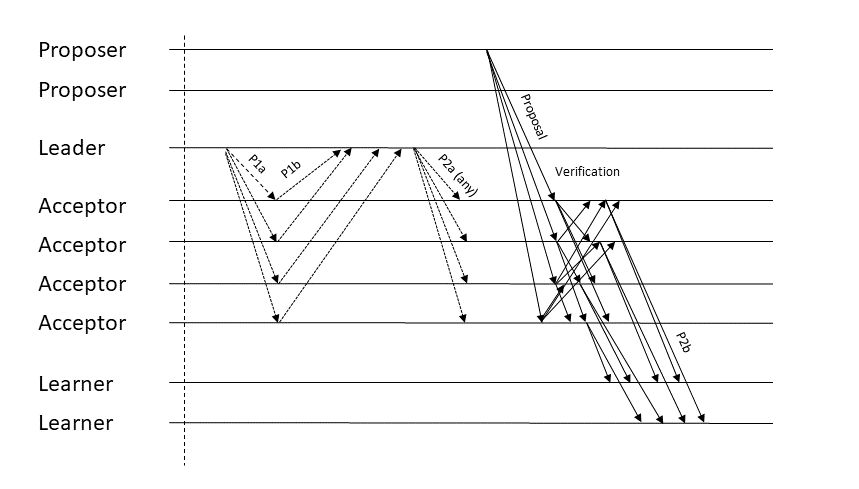
\includegraphics[width=\textwidth*2/3]{Figures/bgp_fast}
	\caption{BGP's fast ballot message pattern}
	\label{bgp_fast}
\end{figure}

In contrast to classic ballots, fast ballots leverage the weaker specification of generalized consensus (compared to classic consensus) in terms of command ordering at different replicas, to allow for the faster execution of commands in some cases.\par
The basic idea of fast ballots is that proposers contact the acceptors directly, bypassing the leader, and then the acceptors send their vote for the current sequence directly to the learners, where this sequence now incorporates the proposed value. If a conflict exists and progress isn't being made, the protocol reverts to using a classic ballot. This is where generalized consensus allows for avoiding falling back to this slow path, namely in the case that the commands that are sequenced in a different order at different acceptors commute. However, this concurrency introduces safety problems even when a quorum is reached for some sequence. If we keep the previous Fast Paxos message pattern, it's possible for one sequence $s$ to be learned at one learner $l_1$ while another non-commutative sequence $s'$ is learned before $s$ at another learner $l_2$. Suppose $s$ obtains a quorum of votes and is learned by $l_1$ but the same votes are delayed indefinitely before reaching $l_2$. In the next classic ballot, when the leader gathers a quorum of $p1b$ messages it must arbitrate an order for the commands that it received from the acceptors and it doesn't know the order in which they were learned. This is because, of the $N-f$ messages it received, $f$ may not have participated in the quorum and other $f$ may be Byzantine and lie about their vote, which only leaves one correct acceptor that participated in the quorum. A single vote isn't enough to determine if the sequence was learned or not. If the leader picks the wrong sequence, it would be proposing a sequence $s'$ that is non-commutative to a learned sequence $s$. Since the learning of $s$ was delayed before reaching $l_2$, $l_2$ would learn $s'$ and be in a conflicting state with respect to $l_1$, violating consistency. {\color{red}In order to prevent this, sequences accepted by a quorum of acceptors must be monotonic extensions of previous accepted sequences. Regardless of the order in which a learner learns a set of monotonic sequences, the resulting state will be the same. The additional verification phase is what allows acceptors to prove to the leader that some sequence was accepted by a quorum. By gathering $N-f$ proofs for some sequence, an acceptor can prove that at least $f+1$ correct acceptors voted for that sequence. Since there are only another $2f$ acceptors in the system, no other non-commutative values can be voted for by a quorum. \par
An interesting alternative to requiring $N-f$ proofs from each acceptor, would be for the leader to wait for $2f+1$ phase $1b$ messages for some sequence. Since at least $f+1$ of those would be correct, only that sequence could've been learned since any other non-commutative sequence would obtain at most $2f$ votes. Zyzzyva uses a similar approach of waiting for $3f+1$ to commit requests in single round-trip in executions where no faults occur~\cite{Kotla:2008}. However, this approach is unsuitable for \acrshort{bgp} since it's possible for a sequence to be chosen by a majority without the leader being aware of more than $f+1$ votes in its quorum. Since $f+1$ votes aren't enough to ensure the leader that the sequence was chosen by a majority, the leader wouldn't be able to pick a learned sequence.}\todo{Improved the explanation but at this point it's not really an introductory paragraph. Should I leave it as is?}\par
Next, we explain each of the protocol's steps for fast ballots in greater detail.

\noindent {\bf Step 1: Proposer to acceptors.}
To initiate a fast ballot, the leader informs both proposers and acceptors that the proposals may be sent directly to the acceptors. Unlike classic ballots, where the sequence proposed by the leader consists of the commands received from the proposers appended to previously proposed commands, in a fast ballot, proposals can be sent to the acceptors in the form of either a single command or a sequence to be appended to the command history. These proposals are sent directly from the proposers to the acceptors.\par

\begin{algorithm} 
	\caption{Byzantine Generalized Paxos - Acceptor a (agreement)}
	\label{BFT-Acc}
	\textbf{Local variables:} $leader = \bot,\ view = 0, bal_a = 0,\ val_a = \bot,\ fast\_bal = \bot,\ proven = \bot$
	\begin{algorithmic}[1]
		\State \textbf{upon} \textit{receive($P1A, ballot, view_l$)} from leader $l$ \textbf{do}
		\State \hspace{\algorithmicindent} \textbf{if} $view_l == view$ and $bal_a < ballot$ \textbf{then}
		\State \hspace{\algorithmicindent}\hspace{\algorithmicindent} $\Call{send}{P1B, ballot,bal_a,proven, val_a, proofs[bal_a]}$ to leader;
		\State \hspace{\algorithmicindent}\hspace{\algorithmicindent} $bal_a = ballot$;	
		\State \hspace{\algorithmicindent}\hspace{\algorithmicindent} $val_a = \bot$;	
		
		
		\State
		\State \textbf{upon} \textit{receive($FAST,ballot,view_l$)} from leader \textbf{do}
		\State \hspace{\algorithmicindent} \textbf{if} $view_l == view$ \textbf{then}
		\State \hspace{\algorithmicindent}\hspace{\algorithmicindent} $fast\_bal[ballot] = true$;

		\State
		\State \textbf{upon} \textit{receive($VERIFY,view_i, ballot_i,val_i,proof$)} from acceptor $i$ \textbf{do}
		\State \hspace{\algorithmicindent} \textbf{if} $proof_{pub_i} == \langle ballot_i, val_i \rangle$ and $view == view_i$ \textbf{then}
		
		\State \hspace{\algorithmicindent}\hspace{\algorithmicindent} $proofs[ballot_i][val_i][i] = proof$;
		\State \hspace{\algorithmicindent}\hspace{\algorithmicindent} \textbf{if} $\#(proofs[ballot_i][val_i]) \geq N-f$ \textbf{then}
		\State \hspace{\algorithmicindent}\hspace{\algorithmicindent}\hspace{\algorithmicindent} $proven = val_i$;
		\State \hspace{\algorithmicindent}\hspace{\algorithmicindent}\hspace{\algorithmicindent} $\Call{send}{P2B, ballot_i, val_i, proofs[ballot_i][value_i]}$ to learners;
		
		\State
		\State \textbf{upon} \textit{receive$(P2A\_CLASSIC, ballot, view, value$)} from leader \textbf{do}
		\State \hspace{\algorithmicindent} \textbf{if} $view_l == view$ \textbf{then}
		\State \hspace{\algorithmicindent}\hspace{\algorithmicindent} \Call{phase\_2b\_classic}{$ballot, value$}; 
		
		\State		
		\State \textbf{upon} \textit{receive($P2A\_FAST, value$)} from proposer \textbf{do}
		\State \hspace{\algorithmicindent} \Call{phase\_2b\_fast}{$value$};
	
		\State
		\Function{phase\_2b\_classic}{$ballot, value$}
		\State $univ\_commut = \Call{isUniversallyCommutative}{val_a}$;
		\State \textbf{if} $ballot \geq bal_a$ and $val_a ==  \bot$ and \ $!fast\_bal[bal_a]$ and ($univ\_commut$ or $proven == \bot$ or $proven == \Call{subsequence}{value, 0, \#(proven)}$) \textbf{then}
		\State \hspace{\algorithmicindent} $bal_a = ballot$;
		\State \hspace{\algorithmicindent} \textbf{if} $univ\_commut$ \textbf{then}
		\State \hspace{\algorithmicindent}\hspace{\algorithmicindent} $\Call{send}{P2B,bal_a, value}$ to learners;
		\State \hspace{\algorithmicindent} \textbf{else} 
		\State \hspace{\algorithmicindent}\hspace{\algorithmicindent} $val_a = value$;
		\State \hspace{\algorithmicindent}\hspace{\algorithmicindent} $proof = \langle ballot, val_a \rangle_{priv_a}$;
		\State \hspace{\algorithmicindent}\hspace{\algorithmicindent} $proofs[ballot][val_a][a] = proof$;
		\State \hspace{\algorithmicindent}\hspace{\algorithmicindent} $\Call{send}{VERIFY, view, ballot, val_a, proof}$ to acceptors;
		\EndFunction
		
		\State
		\Function{phase\_2b\_fast}{$ballot, value$}
		\State \textbf{if} $ballot == bal_a$ and $fast\_bal[bal_a]$ \textbf{then}
		\State \hspace{\algorithmicindent} \textbf{if} $\Call{isUniversallyCommutative}{value}$ \textbf{then}
		\State \hspace{\algorithmicindent}\hspace{\algorithmicindent} $\Call{send}{P2B,bal_a, value}$ to learners;
		\State \hspace{\algorithmicindent} \textbf{else}
		\State \hspace{\algorithmicindent}\hspace{\algorithmicindent} $val_a = val_a \bullet value$;
		\State \hspace{\algorithmicindent}\hspace{\algorithmicindent} $proof = \langle ballot, val_a \rangle_{priv_a}$;
		\State \hspace{\algorithmicindent}\hspace{\algorithmicindent} $proofs[ballot][val_a][a] = proof$;
		\State \hspace{\algorithmicindent}\hspace{\algorithmicindent} \Call{send}{\textit{$VERIFY, view, ballot, val_a, proof$}} to acceptors;
		\EndFunction
	\end{algorithmic}
\end{algorithm}

\noindent {\bf Step 2: Acceptors to acceptors.}
Acceptors append the proposals they receive to the proposals they have previously accepted in the current ballot and broadcast the result to the other acceptors. This broadcast contains a signed tuple of the current ballot and the sequence being voted for and intuitively corresponds to a verification phase where acceptors gather proof that a sequence gathered enough support to be committed. This proof will be sent to the leader in subsequent ballots in order for it to pick a new sequence that preserves consistency. To ensure safety, correct learners must learn non-commutative commands in a total order. When an acceptor gathers $N-f$ proofs for equivalent values, it proceeds to the next phase. That is, sequences do not necessarily have to be equal in order to be learned since commutative commands may be reordered. Recall that a sequence is equivalent to another if it can be transformed into the second one by reordering its elements without changing the order of any pair of non-commutative commands. (Note that, in the pseudocode, proofs for equivalent sequences are being treated as belonging to the same index of the \emph{proofs} variable, to simplify the presentation.) By requiring $N-f$ votes for a sequence of commands, we ensure that, given two sequences where non-commutative commands are differently ordered, only one sequence will receive enough votes even if $f$ Byzantine acceptors vote for both sequences. Outside the set of (up to) $f$ Byzantine acceptors, the remaining $2f+1$ correct acceptors will only vote for a single sequence, which means there are only enough correct processes to commit one of them. Note that the fact that proposals are sent as extensions to previous sequences is critical to the safety of the protocol. In particular, since the votes from acceptors can be reordered by the network before being delivered to the learners, if these values were single commands it would be impossible to guarantee that non-commutative commands would be learned in a total order. \par
\noindent {\bf Step 3: Acceptors to learners.} Similarly to what happens in classic ballots, the fast ballot equivalent of the phase $2b$ message, which is sent from acceptors to learners, contains the current ballot number, the command sequence and the $N-f$ proofs gathered in the verification round. One could think that, since acceptors are already gathering proofs that a value will eventually be committed, learners are not required to gather $N-f$ votes and they can wait for a single phase $2b$ message and validate the $N-f$ proofs contained in it. However, this is not the case due to the possibility of learners learning sequences without the leader being aware of it. If we allowed the learners to learn after witnessing $N-f$ proofs for just one acceptor then that would raise the possibility of that acceptor not being present in the quorum of phase $1b$ messages. Therefore, the leader wouldn't be aware that some value was proven and learned. The only way to guarantee that at least one correct acceptor will relay the latest proven sequence to the leader is by forcing the learner to require $N-f$ phase $2b$ messages since only then will one correct acceptor be in the intersection of the two quorums. \par
\noindent {\bf Arbitrating an order after a conflict.} When, in a fast ballot, non-commutative commands are  concurrently proposed, these commands may be incorporated into the sequences of various acceptors in different orders, and therefore the sequences sent by the acceptors in phase $2b$ messages will not be equivalent and will not be learned. In this case, the leader subsequently runs a classic ballot and gathers these unlearned sequences in phase $1b$. Then, the leader will arbitrate a single serialization for every previously proposed command, which it will then send to the acceptors. Therefore, if non-commutative commands are concurrently proposed in a fast ballot, they will be included in the subsequent classic ballot and the learners will learn them in a total order, thus preserving consistency.
\iffalse \par
\noindent {\bf Quorum intersections.} 
{\color{red} I think this part is wrong. This condition might be unnecessary.}
Another important detail is that acceptors only send their phase $2b$ messages after voting in the verification phase, not only after receiving $N-f$ votes from other acceptors. To understand why this is necessary, note that there are three types of quorums in the protocol: quorums gathered at the leader in phase $1b$, at the acceptors in the verification phase and at the learners in phase $2b$. The leader's quorum needs to intersect with both the verification and the phase $2b$ quorum in order to be sure of proven and unproven sequences, respectively (from now on, sequences for which acceptors received $N-f$ verification votes and therefore sent a vote in a phase $2b$ message are called \textit{proven} sequences). However, it's impossible to have both intersections and still guarantee liveness, because it would require the leader to wait for messages from possibly faulty acceptors. It becomes possible to guarantee this intersection if we force the set of acceptors that participated in phase $2b$ to be contained in the set of acceptors that participated in the verification phase. We ensure that the set of acceptors that participated in the verification phase is a superset of the set of acceptors that participated in phase $2b$ by only allowing an acceptor to vote for phase $2b$ if he has voted for the verification phase in addition to have seen $N-f$ votes.
\fi
\subsubsection{Classic ballots} 

\begin{figure}
	\centering
	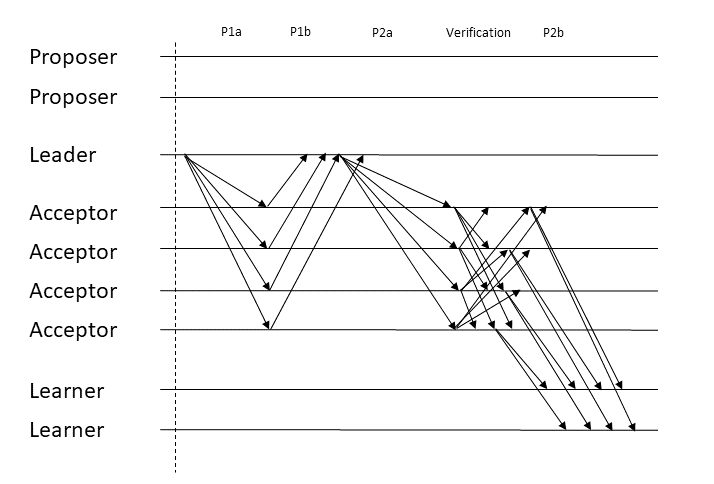
\includegraphics[width=\textwidth*2/3]{Figures/bgp_classic}
	\caption{BGP's classic ballot message pattern}
	\label{bgp_classic}
\end{figure}
Classic ballots work in a way that is very close to the original Paxos protocol~\cite{Lam98}. Therefore, throughout our description, we will highlight the points where \acrshort{bgp} departs from that original protocol, either due to the Byzantine fault model, or due to behaviors that are particular to the specification of Generalized Paxos.

In this part of the protocol, the leader continuously collects proposals by assembling all commands that are received from the proposers since the previous ballot in a sequence. (This differs from classic Paxos, where it suffices to keep a single proposed value that the leader attempts to reach agreement on.)

When the next ballot is triggered, the leader starts the first phase by sending phase $1a$ messages to all acceptors containing just the ballot number. Similarly to classic Paxos, acceptors reply with a phase $1b$ message to the leader, which reports all sequences of commands they voted for. In classic Paxos, acceptors also promise not to participate in lower-numbered ballots, in order to prevent safety violations~\cite{Lam98}. However, in \acrshort{bgp} this promise is already implicit, given (1) there is only one leader per view and it is the only process allowed to propose in a classic ballot and (2) acceptors replying to that message must be in the same view as that leader.

As previously mentioned, phase $1b$ messages contain $N-f$ proofs for each learned sequence. By waiting for $N-f$ such messages, the leader is guaranteed that, for any learned sequence $s$, at least one of the messages will be from a correct acceptor that, due to the quorum intersection property, participated in the verification phase of $s$. In the \acrshort{cft} version of the protocol, the leader could determine if some value had been chosen by a majority of acceptors by looking for $f+1$ identical votes in the quorum of phase $1b$ messages. If some value had $f+1$ votes, no other value could have been chosen since there are only other $2f$ acceptors in the system. However, the same isn't true for \acrshort{bgp} because $f+1$ identical votes for some value only attest that at least one correct process voted for that value. It's impossible to determine if some value was chosen by a majority unless a correct process witnesses $2f+1$ identical votes. Note that, since each command is signed by the proposer (this signature and its check is not explicit in the pseudocode), a Byzantine acceptor can't relay made-up commands. However, it can omit commands from its phase $1b$ message, which is why it's necessary for the leader to be sure that at least one correct acceptor in its quorum took part in the verification quorum of any learned sequence. \par
After gathering a quorum of $N-f$ phase $1b$ messages, the leader initiates phase $2a$ where it assembles a proposal and sends it to the acceptors. This proposal sequence must be carefully constructed in order to ensure all of the intended properties. In particular, the proposal cannot contain already learned non-commutative commands in different relative orders than the one in which they were learned, in order to preserve consistency, and it must contain unlearned proposals from both this and the previous ballots, in order to preserve liveness (this differs from sending a single value with the highest ballot number as in the classic specification). Due to the importance and required detail of the leader's value picking rule, it will be described next in its own section. The acceptors reply to phase $2a$ messages by broadcasting their verification messages containing the proposed sequence and proof of their committal to that sequence. After receiving $N-f$ verification messages, an acceptor sends its phase $2b$ message to the learners, containing the ballot, the proposal from the leader and the $N-f$ proofs gathered in the verification phase. As is the case in fast ballot, when a learner receives a phase $2b$ vote, it validates the $N-f$ proofs contained in it. Waiting for a quorum of $N-f$ messages for a sequence ensures the learners that at least one of those messages was sent by a correct acceptor that will relay the sequence to the leader in the next classic ballot. (The learning of sequences also differs from the original protocol in the quorum size, due to the fault model, and in that the learners would wait for a quorum of matching values instead of equivalent sequences, due to the consensus specification.)\par

\noindent {\bf Leader value picking rule.} Phase $2a$ is crucial for the correct functioning of the protocol because it requires the leader to pick a value that allows new commands to be learned, ensuring progress, while at the same time preserving a total order of non-commutative commands at different learners, ensuring consistency. The value picked by the leader is composed of three pieces: (1) the subsequence that has proven to be accepted by a majority of acceptors in the previous fast ballot, (2) the subsequence that has been proposed in the previous fast ballot but for which a quorum hasn't been gathered and (3) new proposals sent to the leader in the current classic ballot. \par
The first part of the sequence will be the largest sequence of the $N-f$ proven sequences sent in the phase $1b$ messages. The leader can pick such a value deterministically because, for any two proven sequences, they are either equivalent or one can be extended to the other. The leader is sure of this because for the quorums of any two proven sequences there is at least one correct acceptor that voted in both and votes from correct acceptors are always extensions of previous votes from the same ballot. If there are multiple sequences with the maximum size then they are equivalent (by same reasoning applied previously) and any can be picked. \par
The second part of the sequence is simply the concatenation of unproven sequences or commands in an arbitrary order. Since these commands are guaranteed to not be learned at any learner, they can be appended to the leader's sequence in any order. Since $N-f$ phase $2b$ messages are required for a learner to learn a sequence and the intersection between the leader's quorum and the quorum gathered by a learner for any sequence contains at least one correct acceptor, the leader can be sure that if a sequence of commands is unproven in all of the gathered phase $1b$ messages, then that sequence wasn't learned and can be safely appended to the leader's sequence in any order. \par 
The third part consists simply of commands sent by proposers to the leader with the intent of being learned at the current ballot. These values can be appended in any order and without any restriction since they're being proposed for the first time.

\begin{algorithm}
	\caption{Byzantine Generalized Paxos - Learner l}
	\label{BFT-Learn}
	\textbf{Local variables:} $learned = \bot, messages = \bot$
	\begin{algorithmic}[1]			
		\State \textbf{upon} \textit{receive($P2B, ballot, value, proofs$)} from acceptor $a$ \textbf{do}
		\State \hspace{\algorithmicindent} $valid\_proofs = 0$;
		\State \hspace{\algorithmicindent} \textbf{for} $i$ \textbf{in} $acceptors$ \textbf{do}
		\State \hspace{\algorithmicindent}\hspace{\algorithmicindent} $proof = proofs[i]$;
		\State \hspace{\algorithmicindent}\hspace{\algorithmicindent} \textbf{if} $proof_{pub_i} == \langle ballot, value \rangle$ \textbf{then}
		\State \hspace{\algorithmicindent}\hspace{\algorithmicindent}\hspace{\algorithmicindent} 
		$valid\_proofs \mathrel{+{=}} 1$;
		\State
		\State \hspace{\algorithmicindent} \textbf{if} $valid\_proofs \geq N-f$ \textbf{then}
		\State \hspace{\algorithmicindent}\hspace{\algorithmicindent} $messages[ballot][value][a] = proofs$;
		\State
		\State \hspace{\algorithmicindent}\hspace{\algorithmicindent} \textbf{if} $\#(messages[ballot][value]) \geq N-f$ \textbf{then}
		\State \hspace{\algorithmicindent}\hspace{\algorithmicindent}\hspace{\algorithmicindent} $learned = \Call{merge\_sequences}{learned, value}$;

		\State
		\State \textbf{upon} \textit{receive($P2B, ballot, value$)} from acceptor $a$ \textbf{do}
		\State \hspace{\algorithmicindent} \textbf{if} $\Call{isUniversallyCommutative}{value}$ \textbf{then}
		\State \hspace{\algorithmicindent}\hspace{\algorithmicindent}
		 $messages[ballot][value][a] = true$;
		\State \hspace{\algorithmicindent}\hspace{\algorithmicindent} \textbf{if} $\#(messages[ballot][value]) > f$ \textbf{then} 
		\State \hspace{\algorithmicindent}\hspace{\algorithmicindent}\hspace{\algorithmicindent} $learned = learned \bullet value$;
		
		\State		
		\Function{merge\_sequences}{$old\_seq, new\_seq$}
		\State \textbf{for} $c$ \textbf{in} $new\_seq$ \textbf{do} 
		\State \hspace{\algorithmicindent} \textbf{if} $!\Call{contains}{old\_seq,c}$ \textbf{then}
		\State \hspace{\algorithmicindent}\hspace{\algorithmicindent}\hspace{\algorithmicindent} $old\_seq =  old\_seq \bullet c$;
		\State \textbf{return} $old\_seq$;
		\EndFunction
	\end{algorithmic}
\end{algorithm}

\subsubsection{Byzantine leader}
The correctness of the protocol is heavily dependent on the guarantee that the sequence accepted by a majority of acceptors if a prefix of subsequent proven sequences. Otherwise, if the network rearranges phase $2b$ messages such that they're seen by different learners in different orders, they will result in a state divergence. If, however, every vote is a prefix of all subsequent votes then, regardless of the order in which the sequences are learned, the final state will be the same. \par 
This state equivalence between learners is ensured by the correct execution of the protocol since every vote in a fast ballot is equal to the previous vote with a sequence appended at the end and every vote in a classic ballot is equal to all the learned votes concatenated with unlearned votes and new proposals which means that new votes will be extensions of previous proven sequences. However, this begs the question of how the protocol fares when Byzantine faults occur. In particular, the worst case scenario occurs when both $f$ acceptors and the leader are Byzantine (remember that a process can have multiple roles, such as leader and acceptor). In this scenario, the leader can purposely send phase $2a$ messages for a sequence that is not prefixed by the previously accepted values. Coupled with an asynchronous network, this malicious message can be delivered before the correct votes of the previous ballot, resulting in different learners learning different sequences that may not be extensible to equivalent sequences. \par
To prevent this scenario, the acceptors must ensure that the proposals they receive from the leader are prefixed by the values they have previously voted for. Since an acceptor votes for its $val_a$ sequence after receiving $N-f$ verification votes for an equivalent sequence and stores it in its $proven$ variable, the acceptor can verify that it is an eq-prefix of the leader's proposed value (i.e., $proven \sqsubseteq value$). A practical implementation of this condition is simply to verify that the  subsequence of $value$ starting at the index $0$ up to index $length(proven)-1$ is equivalent to the acceptor's $proven$ sequence. 

\subsection{Discussion}

\subsubsection{Handling faults in the fast case.}
A result that was stated in the original Generalized Paxos paper~\cite{Lamport2005} is that to tolerate $f$ crash faults and allow for fast ballots whenever there are up to $e$ crash faults, the total system size $N$ must uphold two conditions: $N > 2f$ and $N > 2e+f$. Additionally, the fast and classic quorums must be of size $N-e$ and $N-f$, respectively. This implies that there is a price to pay in terms of number of replicas and quorum size for being able to run fast operations during faulty periods. An interesting observation is that since Byzantine fault tolerance already requires a total system size of $3f+1$ and a quorum size of $2f+1$, we are able to amortize the cost of both features, i.e., we are able to tolerate the maximum number of faults for fast execution without paying a price in terms of the replication factor and quorum size.

\subsubsection{Universally commutative commands}
In the \acrshort{cft} version of the protocol, we mentioned that a downside of taking advantage of commutative commands to reduce synchronization requirements is that the commutativity check must be done at runtime. However, a possible extension to the protocol considers sequences that don't require the check to be performed because they are certain to be commutative with any other sequence. This extension allows us to optimize the protocol both by bypassing the verification round and by allowing learners to learn these universally commutative sequences after witnessing a reduced quorum of $f+1$ learners since there are no possible conflicts with other sequences. Furthermore, this reduced quorum is enough for a learner be sure that the proposal was proposed by a valid proposer. This extension would also optimize the protocol's performance in a geo-replicated setting because there could be a significant latency reduction between waiting for the fastest $f+1$ acceptors and the fastest $N-f$.\par
{\color{red} Much like the equivalent extension to the \acrshort{cft} protocol, the usefulness of this optimization is severely reduced if these sequences are treated like any other at the leader and acceptors. This is due to the fact that new proposals are appended to sequences that are proven to have been accepted by a majority. Since these proven sequences are probably not universally commutative, the resulting sequence will not be as well. As in the previous protocol, we can increase its applicability by sending these sequences immediately to the learners, without appending them to previously accepted ones. However, in \acrshort{bgp} this special handling has the added benefit of bypassing the verification phase, resulting in latency for the requests and less traffic generated per sequence. This extension can also be easily implemented by adding a single check in Algorithm \ref{BFT-Lead} lines \{19-20\}, Algorithm \ref{BFT-Acc} lines \{29-30,40-41\} and Algorithm \ref{BFT-Learn} lines \{14-18\}.}

\subsubsection{Checkpointing}  \acrshort{bgp} includes an additional feature that allows the leader to propose a special command $C^*$ that causes both the acceptors and learners to safely discard previously stored commands. This feature is of great practical importance since it can be used to prevent commands from being stored indefinitely. However, the reason why acceptors accumulate state continuously is because each new proven sequence must contain any previously accepted proven sequence. This ensures that neither the network nor Byzantine agents can reorder messages and cause learners to learn in different orders. In order to safely discard state at the acceptors, they must be sure that every learner has learned the proven commands up to a certain agreed upon point. The simplest way of guaranteeing this is having the leader determine when to initiate the checkpointing subprotocol and, in its next proposal, include a special checkpointing command $C^*$. When learned by a learner, this special command prompts the learner to discard every learned command up to (but not including) $C^*$ and send a message to the acceptors acknowledging its existence. This acknowledgment carries with it a proof that the learner has discarded its state and consists in a digital signature of the command with the learner's public key. After receiving acknowledgments from every learner, an acceptor discards every previous command up to $C^*$. \par
As with non-checkpointing sequences, there is a sequence that contains the checkpointing command being witnessed by learners in an order different than the one that they were intended to be learned in. Usually, safety is ensured because every subsequent proposal is an extension of previous ones.{\color{red} However, since the checkpointing prompts both the acceptors and the learners to discard the sequences they hold, it's possible for a delayed sequence to be executed after the checkpointing command. Usually, this delayed sequence would be included in subsequent sequences as a prefix, such that the learner already had witnessed those commands. When the delayed message got to the learner, those commands would already be incorporated in learner's learned sequence of commands $learned_l$ and the state wouldn't change. However, after executing the checkpointing command, the state is empty which means that the duplicate commands in the delayed message wouldn't be detected. To avoid delayed messages from causing commands to be executed multiple times, it's critical that both the acceptors and the learners discard every learned command except the command $C^*$ that prompted the state to be discarded.} By retaining this command, the learners can check that subsequent sequences do not contain commands learned before the checkpointing step by requiring that they begin with $C^*$. Since the acceptors also leave the checkpointing command in their sequence of proven commands, every valid subsequent sequence will begin with $C^*$. This extension to the protocol isn't included in the pseudocode due to space constraints.

\subsubsection{Fast Byzantine Paxos comparison}
In comparison to \acrshort{fab} Paxos, our \acrlong{bgp} protocol requires a lower number of acceptors than what is stipulated by \acrshort{fab}'s lower bound~\cite{Martin2006}. However, this does not constitute a violation of the result since BGP does not guarantee a two step execution in the Byzantine scenario. Instead, \acrshort{bgp} only provides a two communication step latency when proposed sequences are universally commutative with any other sequence. In the common case, \acrshort{bgp} requires three messages steps for a sequence to be learned. In other words, Byzantine Generalized Paxos introduces an additional broadcast phase to decrease the requirements regarding the minimum number of acceptor processes. This may be a sensible trade-off in systems that target datacenter environments where communication between machines is fast and a high percentage of costs is directly related to equipment since fast communication links mitigate the latency cost of having an additional phase between the acceptors and the high cost of equipment and power consumption makes the reduced number of acceptor processes attractive.